\chapter{Evaluation und Validation}
\label{ch:evaluation}

% Auswertung und Interpretation der Ergebnisse. Nachweis, dass die Ziele erreicht wurden, oder
% warum welche nicht erreicht wurden.

In diesem Kapitel werden nun die Ergebnisse dieser Arbeit ausgewertet.
Im ersten Abschnitt \fullref{sec:messresultate} werden die Messungen
ausgewertet.
Anschliessend werden im Abschnitt \fullref{sec:vergleich_anforderungen}

\section{Messresultate}\label{sec:messresultate}

Als Erstes wurde die Testumgebung überprüft, ob diese überhaupt sinnvolle Resultate misst.
Anschliessend wurden zwei verschiedene Arten von Messungen durchgeführt.
Für weitere Messungen, vor allem für Messungen mit Bandbreitenbeschränkung, war die Zeit leider zu knapp.

Bei jeder Messung wurden 1000 Nachrichten von einem zufälligen Knoten verschickt
und von einem anderen zufälligem Knoten im Testnetzwerk wieder empfangen.
Zudem wurde die konfigurierte Tunnellänge bei jeder Messung auf dem Standardwert \lstinline|3| belassen.
Die Nachrichten wurden jeweils in einem Abstand von sechs Sekunden nacheinander verschickt,
damit das Netzwerk auf keinen Fall überlastet wird.
Zudem wurde jeweils die CPU-Ressourcenauslastung und Netzwerkbelastung alle 5-Sekunden gemessen.

\subsection{Validation der Testumgebung}\label{sec:validation_testumgebung}

Um Aussagen machen zu können über das Testnetzwerk und deren Messresultate, muss erst sichergestellt werden, dass die Messwerte überhaupt Sinn ergeben.
Deshalb wurden erste Messungen und Tests durchgeführt, um zu prüfen, ob die Testumgebung auch richtig funktioniert.
% Um sicherzustellen, dass kein Fehler beispielsweise im implementieren Testnetzwerk oder gar in der i2pd-Software aufzufinden ist, wird diese Messung zu Validierungszwecken durchgeführt.

Als Teil dieser Messung wird erst ein Netzwerk mit 8 Knoten getestet und die Latenz von 1000 Nachrichten gemessen.
Alle Knoten haben in diesem Test keine Bandbreitenbeschränkung.
Die Konfigurierte Nachrichtengrösse wurde jeweils auf 64kB festgelegt.

Als erstes wurde die Messumgebung auf meinem Laptop (8 Kerne, Intel Core i7-8550U CPU @ 1.80GHz, mit 16GB RAM),
getestet mit 8 Knoten und dieselbe Messung mehrfach wiederholt.
Dies hatte jeweils fast immer dasselbe Resultat zur Folge:
Die Nachrichten wurden mit einer Latenzzeit von etwas mehr als fünf Sekunden empfangen.
Einige Ausreisser waren jedoch zu beobachten.
Denn bei manchen Nachrichten liess sich eine Latenzzeit von etwas mehr als sechs Sekunden oder bis hin zu einem vielfachen von fünf Sekunden beobachten.

Anschliessend wurde eine Virtuelle Maschine beim Anbieter Hetzner (16 Kerne, AMD EPYC @ 2.495 GHz, mit 32GB RAM) bestellt, um dort die Messungen durchzuführen.
Alle weiteren Messungen wurden auf dieser Maschine durchgeführt.
Auch dort lieferte derselbe Testaufbau auch bei wiederholten Messungen dieselben Resultate.
Die Nachrichten wurden mit einer Latenzzeit von etwas mehr als fünf Sekunden empfangen
und dieselben Ausreisser (jedoch nicht ganz so häufig) von sechs Sekunden Nachrichten bis hin zu einem vielfachen von fünf Sekunden konnten beobachtet werden.
Somit ist sichergestellt, dass die Messungen wiederholbar und reproduzierbar sind und bieten eine Basis und Referenzpunkt für weitere Messungen \seereq{TREP}.

% \subsection{Wiederholbarkeit von Messungen}
%
% Eine Nachricht wird hier jeweils von einem zufälligen Knoten an einen anderen zufälligen Knoten versendet.
% Die Konfigurierte Nachrichtengrösse wurde jeweils auf 64kB festgelegt.
% Die Messung wird so festgehalten.
% Anschliessend wird derselbe Test noch einmal gestartet, wobei das Testnetzwerk jedoch aber neu erstellt wird.
%
% Grundsätzlich wird hier erwartet, dass die Messungen vergleichbar sind und ähnliche Resultate liefern.
%
% Somit kann ausgesagt werden das die Messungen so gut wie möglich reproduzierbar sind \seereq{TREP}.


\subsection{Gleichbleibende Latenz bei Skalierung des Netzwerks}\label{sec:messung_latenz}

Um nun die Hypothese \ref{hyp:first} zu bearbeiten wird nun als Erstes die Anzahl Knoten skaliert
und mehrmals unter gleichen Bedingungen gemessen.
Die konfigurierte Nachrichtengrösse wurde jeweils auf 64KB festgelegt.
Es wird angenommen, dass sich die Latenz der Nachrichten im Netzwerk nicht hier verändert.
Dies mag auf den ersten Anschein der Hypothese wiedersprechen, jedoch gilt es zu beachten, dass hier alle Knoten dieselbe Bandbreitenbeschränkung von \lstinline|100000| KB/s haben.
Dementsprechend müsste die Peer-Selektion von I2P alle Knoten gleich bewerten.
Der einzige Unterschied zwischen einem kleineren Netzwerk und einem grösseren Netzwerk ist somit lediglich,
dass eine grössere Auswahl an Knoten besteht, an denen eine Nachricht weitergeleitet werden kann.
Die Erwartung ist also, dass somit die Latenz bei steigender Anzahl Knoten gleich bleibt.

\begin{figure*}[htp]
  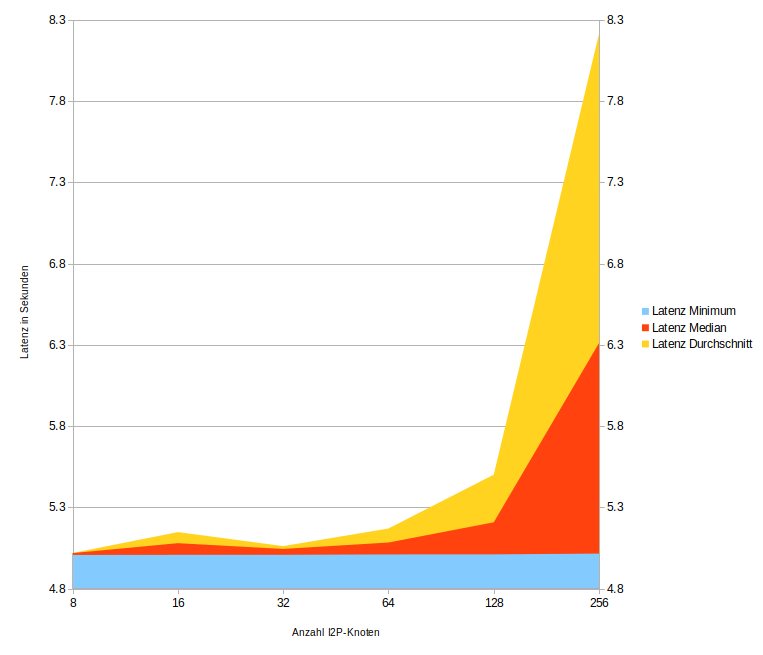
\includegraphics[width=1.1\textwidth]{img/auswertung-latenz.png}
  \caption{Nachrichtenlatenz bei Skalierung der Anzahl I2P-Knoten}\label{fig:auswertung-latenz}
\end{figure*}


Die Abbildung~\fullref{fig:auswertung-latenz} zeigt jedoch ein leicht anderes Bild.
Während die Mindestlatenz der 1000 Nachrichten konstant auf fünf Sekunden bleibt, vergrössert sich die Median- und Durchschnittslatenz je mehr Knoten im Testnetzwerk vorhanden sind.
Vor allem bei einem Netzwerk von 256 Knoten steigt diese beträchtlich an.
Dies ist ein überraschendes Ergebnis und die Gründe sind unklar.
Es könnte sein, dass das man hier auf gewisse implizite Limits im Linux-Kernel bei dieser Menge an Docker-Container gestossen sind.
Jedoch ist die CPU-Auslastung im gemessenen fünf Sekunden Abstand nie auf mehr als 20\% angestiegen und im Schnitt betrug diese lediglich 5\%.


\subsection{Verhalten der Latenz abhängig von der Nachrichtengrösse}\label{sec:messung_nachrichtengroesse}

Bei dieser Messung wurden in einem Testnetzwerk bestehend aus 64 Knoten verschieden grosse Nachrichten versandt.
Auch hier haben alle Knoten dieselbe Bandbreitenbeschränkung von \lstinline|100000| KB/s.
Hier wurde erwartet, dass sich die Latenz unter Umständen leicht vergrössert. Dies aufgrund von Zwischenpuffergrössen wie auch dem zusätzlichen Verschlüsselungsoverhead.

\begin{figure*}[htp]
  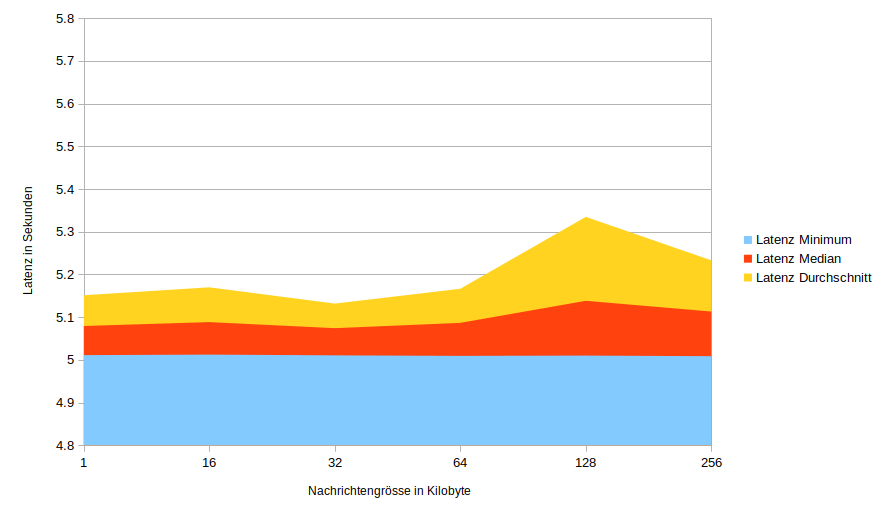
\includegraphics[width=1.1\textwidth]{img/auswertung-nachrichtengroesse.png}
  \caption{Nachrichtenlatenz bei verschiedener Nachrichtengrösse}\label{fig:auswertung-nachrichtengroesse}
\end{figure*}

Wie aus der Grafik~\fullref{fig:auswertung-nachrichtengroesse} zu erkennen ist, verändert sich die Latenz nicht markant anhand der Nachrichtengrösse.
Ein kleiner Anstieg der Latenz ist jedoch ab der Nachrichtengrösse von 64KB ersichtlich.
Jedoch macht dies keinen grossen Unterschied, vor allem auch wenn die Nachrichtengrösse vervierfacht wird auf 256KB, scheint dies keinen grossen Einfluss auf die Latenz zu haben.
Es wurde in diesem Falle sogar eine tiefere Median- und Durchschnittslatenz gemessen, als mit einer Nachrichtengrösse von 128KB.
Es wird angenommen der Grund dafür besteht in der Zwischenpuffergrösse, welche bei I2P ebenfalls auf 64KB gesetzt ist.

\section{Vergleich mit Anforderungen}\label{sec:vergleich_anforderungen}

Es wurde ein Stand der Technik ermittelt \seereq{SDTF} und anhand dessen ein Konzept im Kapitel \fullref{ch:ideen_und_konzepte} \seereq{TKON} erstellt und ein Teststand aufgebaut \seereq{TINF}.
Es wurde darauf geachtet und geprüft ob die Messungen reproduzierbar sind \seereq{TREP}.
Es ist möglich den Teststand und die Messungen zu konfigurieren, wie beschrieben im Abschnitt \fullref{sec:konfigurationsoptionen} \seereq{TCNF}.
Dabei kann man den Teststand auf bis zu 256-Knoten skalieren \seereq{TSCL},
wie beschrieben im Abschnitt \fullref{sec:scaling} und gezeigt bei der Messung im Abschnitt \fullref{sec:messung_nachrichtengroesse}.
Dabei ist das interne I2P-Netzwerk vom realen Testnetzwerk abgeschottet \seereq{TISO} wie beschrieben im Abschnitt \label{sec:netzwerkisolation}.
Optional hätten auch Tests im öffentlichen I2P-Netzwerk durchgeführt werden können \seereq{TNET}.
An verschiedenen Stellen im Programmcode wurde dies vorgesehen und angedacht, dass dies in Zukunft möglich wäre.
Jedoch wird dies nicht komplett unterstützt und wurde auch nie getestet.
Es wurde eine Messanlage entwickelt zur Latenzmessung \seereq{TLAT}
Es wurde die Möglichkeit implementiert die Bandbreite der einzelnen I2P-Knoten zu limitieren \seereq{TLIM}, jedoch wurde diese aus Zeitgründen nie komplett für Messungen eingesetzt und die anderen Experimente hatten Vorrang.
Es ist schnell möglich ein neues Mess-Experiment zu starten \seereq{TVRS}. Es muss lediglich die Konfiguration angepasst werden und die Knoten neu erstellt werden. Im besten Falle ist dies innerhalb von 5 Minuten möglich. Sollte jedoch etwas anderes als eine Latenzmessung durchgeführt werden, müsste die Messanlage angepasst werden. Dies würde weitere Entwicklungsaufwand mit sich bringen.
Es wurde eine Evaluation und Auswertung der Messresultate \seereq{EVAL} im Abschnitt \fullref{sec:messresultate} vorgenommen.
Die Ausführungszeiten der Tests wurden so gut wie möglich kurz gehalten \seereq{TPER}. Eine Messung mit 1000 Nachrichten dauert fast zwei Stunden, da die Nachrichten im Abstand von sechs Sekunden verschickt werden, um das Netzwerk nicht zu überlasten. Andere Experimente könnten hier eine bessere Test-Performance mit sich bringen.

Es wurde mit KanBan ein iteratives Projektmangement eingesetzt \seereq{ITER}. Oft aber hatte man zu viel Overhead mittels Meeting-Notizen.
Zudem wurde als Bestandteil der Bachelorarbeit dieser Bericht erstellt \seereq{DOCS}, eine Zwischenpräsentation gehalten \seereq{PRES}, ein Web-Abstract erstellt, sowie \seereq{WEBA} und ein dazugehöriges Pitching-Video produziert \seereq{PVID}.
Somit konnten meisten Anforderungen erfüllt werden, inklusive den optionalen Anforderungen.

\section{Technische Aspekte}

Mit der Umstellung von der NixOS basierten Lösung auf die auf \lstinline|docker-compose| basierende Lösung ist
die Möglichkeit I2P-Knoten auf mehrere Maschinen zu deployen verloren gegangen.
Denn die Docker-Container werden mit \lstinline|docker-compose| so nur auf einem einzelnen Rechner erstellt und
es können nicht ohne weiteres mehrere Testnetzwerke miteinander verbunden werden.
Mit diesem Ansatz kann nicht auf beliebig viele Knoten skaliert werden, da nur vertikal skaliert werden kann.
Dementsprechend ist dieser Ansatz durch existierende Hardware limitiert.

Für die Messanlage wurde ein eigener TCP-Server und TCP-Client in C-Implementiert, um genauere Messresultate zu erhalten.
Dies hat jedoch viel Zeit beansprucht und eine einfachere Lösung hätte
eventuell ähnlich genaue Resultate liefern können.
Die Auswertung der CSV-Dateien mit den Messresultaten mittels LibreOffice Calc (Excel-pendant) war nicht unbedingt einfach und mühsam. Vor allem hatte ich Probleme beim erstellen der Diagramme. Jedoch war dieses Vorgehen wohl aus Zeitgründen pragmatisch.

Zur Erstellung des Berichts und der Präsentation wurde die \LaTex-Suite eingesetzt. Dies hatte den Vorteil das ich stets in meinem Liebligseditor Vim arbeiten konnte. Zudem bietet \LaTe  mit BibiTex eine Lösung zur Verwaltung von Quellen für eine Literaturverzeichnis und macht das Handhaben jedglicher Referenzen einfach. Weil es sich um reinen Text handelt, konnte auch die Versionsverwaltung Git für den Bericht eingesetzt werden.
Nachteil dieser Lösung ist jedoch, das die Rechtschreibprüfung von Vim nicht so gut ist wie die Rechtschreibprüfung von Word. Dies hat einen Mehraufwand verursacht. Zudem musste oft im Internet nach passenden Befehlen und Paketen gesucht werden, um gewisse Teile des Berichts zu gestalten.
Jedoch konnte ich einiges dazulernen und einen schön gestalteten Bericht abliefern.


\section{Vorgehen}

Die verwendete Projektmangement-Methode von KanBan war sicherlich hilfreich,
auch wenn man sich nicht immer strikt daran gehalten hat oder konnte.
Im Nachhinein hätte man, den einen oder anderen Punkt mehr zu Herzen nehmen sollen.
Zum Beispiel, dass man nicht gleichzeitig an mehreren Sachen arbeiten hätte sollen.
Oft hat man sich während der Entwicklung auch überstürzt und zu viele Änderungen auf einmal vorgenommen, dass nicht mehr klar war wieso etwas nun nicht mehr funktionierte.
Die wöchentlichen Meetings waren extrem hilfreich den Kurs des Projektes zu steuern und schnell Feedback einzuholen.
Oft hat man sich im Detail verloren, sich zu viel vorgenommen, oder überstürzt gehandelt.
Dies konnte durch die Meetings jeweils etwas reguliert werden.
Während die erstellten Meeting-Notizen hilfreich waren, haben diese aber auch oft zu viel Projektmangement-Overhead geführt.

